\section{Quality of Results}

This subchapter addresses the seven questions presented at the end of Chapter \ref{section:goal_and_scope}.

% Do models correctly integrate with third-party software such as Blender \cite{blender}?
\textbf{Q1}:
The generated city models import correctly into Blender.
However, integration with other third-party tools needs to be tested more thoroughly as Blender was the main tool used in this project for verifying the correctness of the exported models.

Although these models are imported correctly in terms of data and structure, there still exist some undesired visual differences.
These differences are, however, a consequence of the difference in rendering pipelines between Unity and any other third-party tool.
Figure~\ref{fig:blender_unity_comparison} showcases these visual differences with Blender.

\begin{figure}[H]
  \centering
  \begin{subfigure}[b]{0.48\textwidth}
    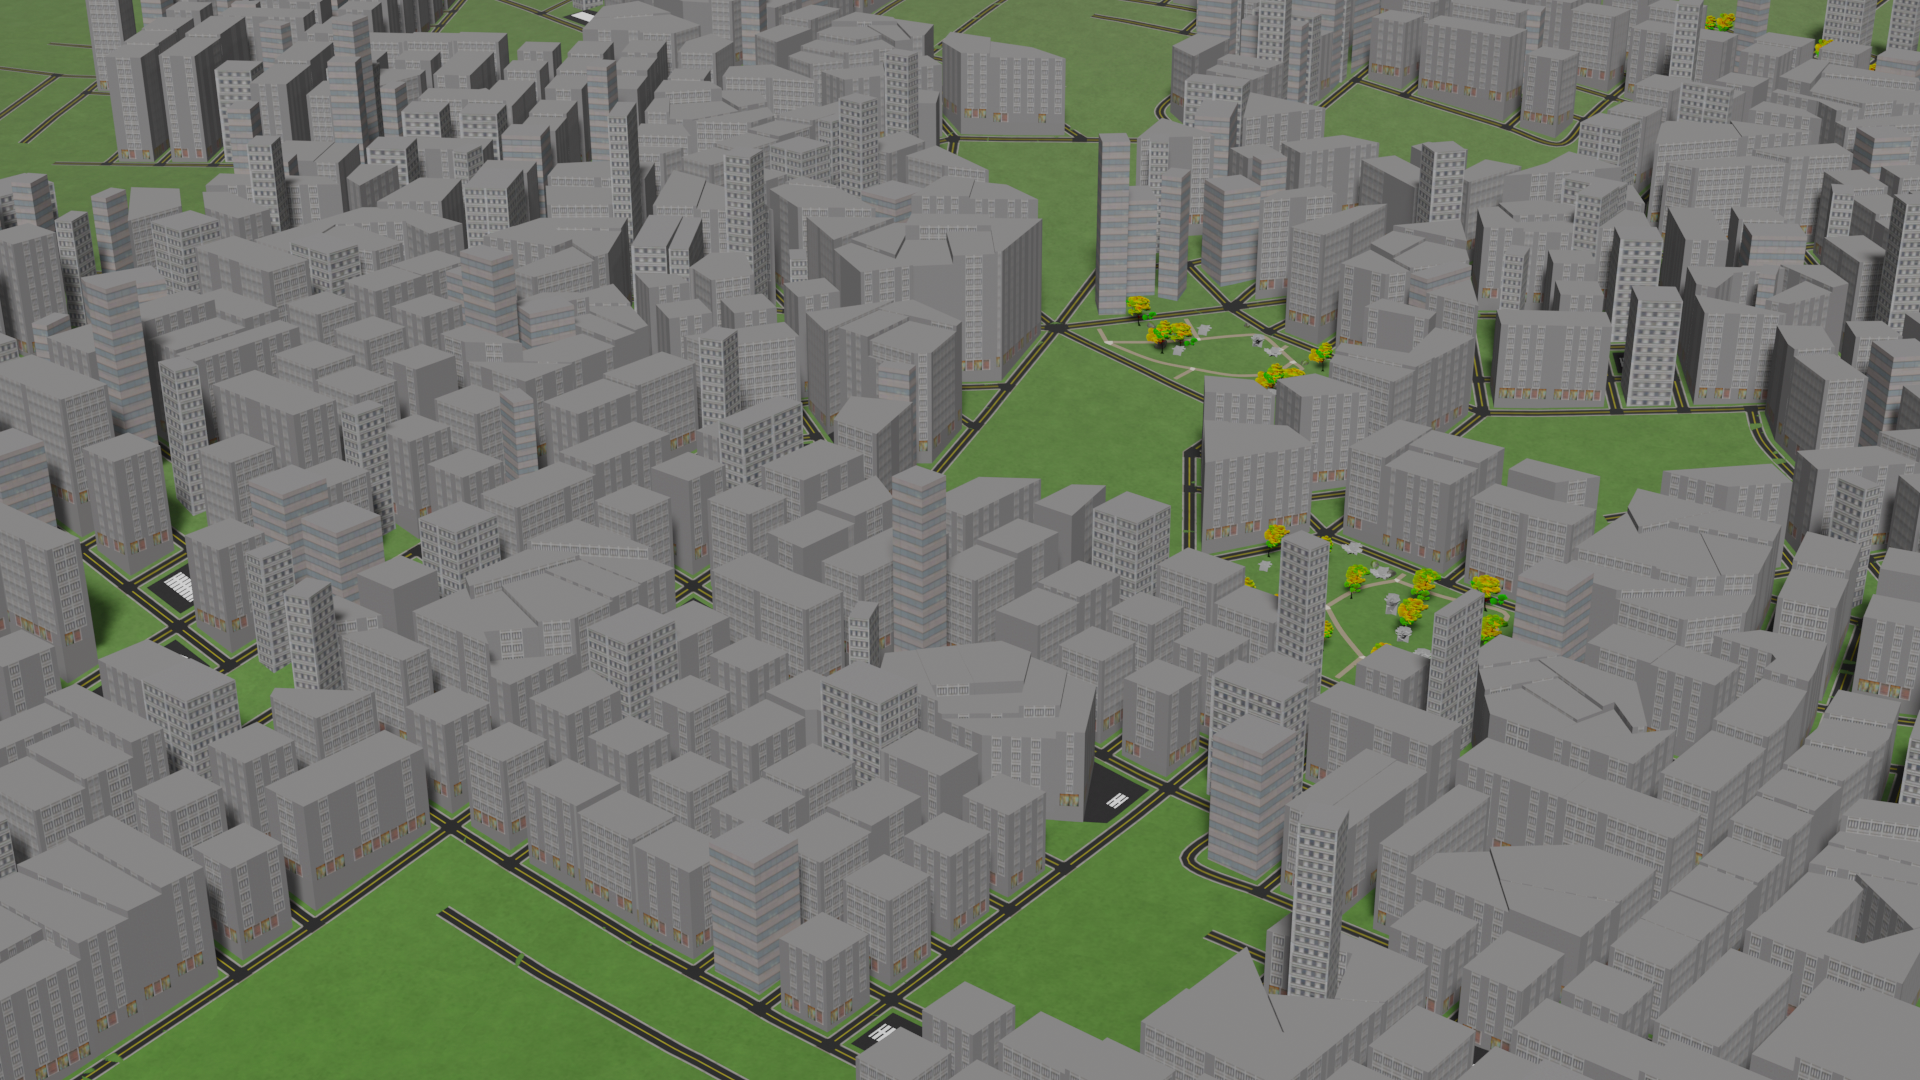
\includegraphics[width=\textwidth]{figure/blender_unity_comparison_blender}
    \caption{CityCraft scene rendered in Blender.}
  \end{subfigure}
  \quad
  \begin{subfigure}[b]{0.48\textwidth}
    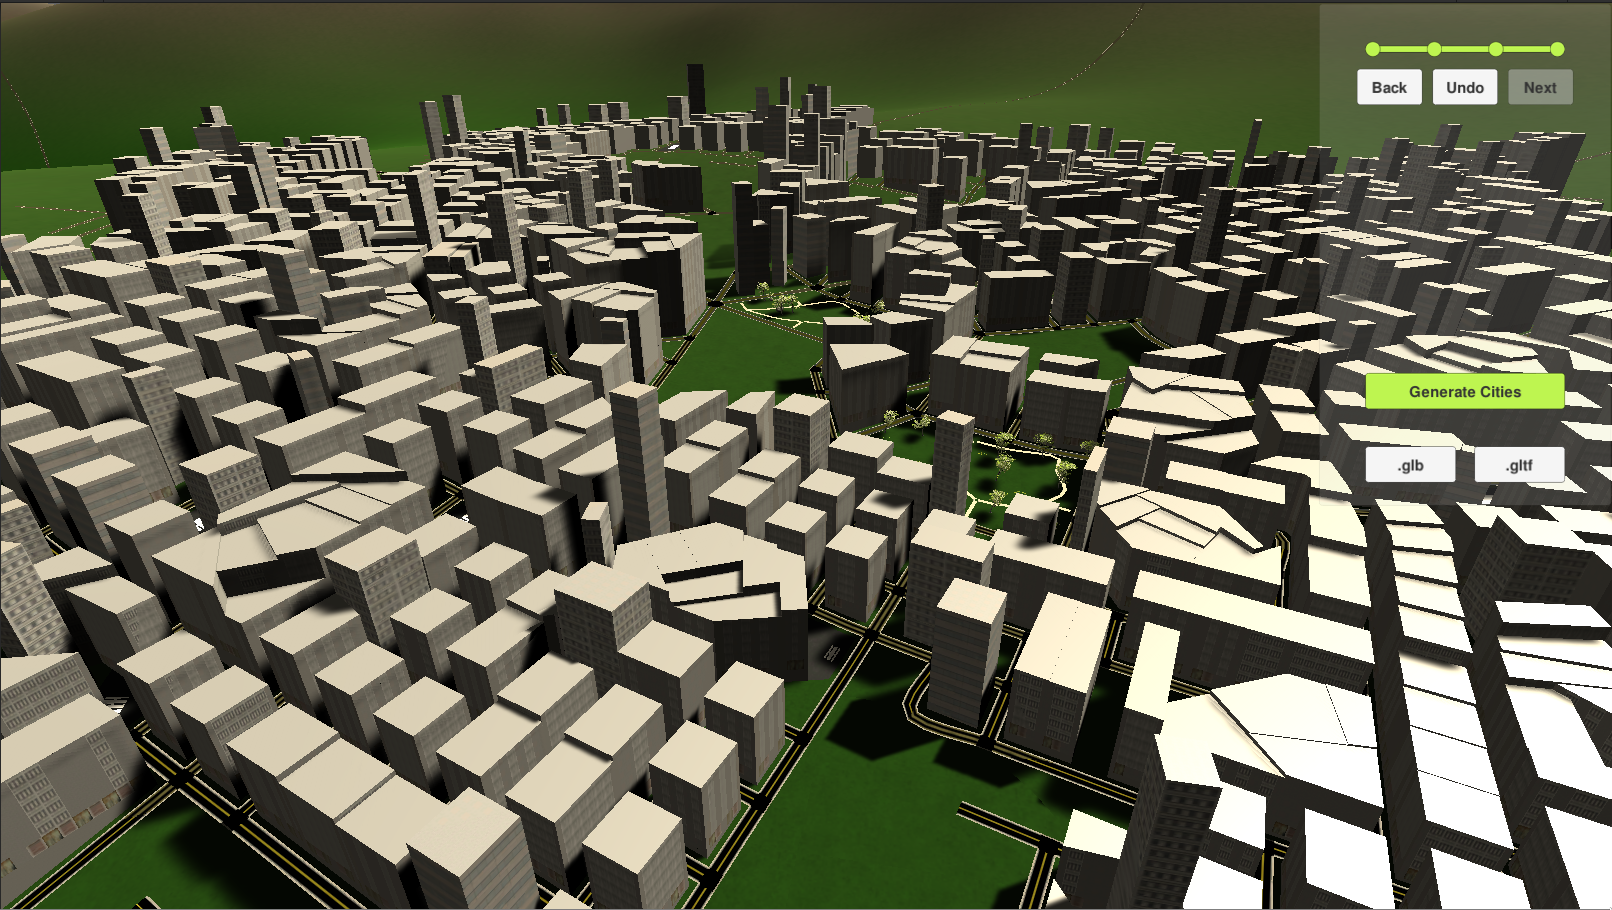
\includegraphics[width=\textwidth]{figure/blender_unity_comparison_unity}
    \caption{CityCraft scene rendered in Unity.}
  \end{subfigure}
  \caption{Visual differences of cities when rendering in Blender and Unity.}
  \label{fig:blender_unity_comparison}
\end{figure}

Importing a generated city into Blender also takes a substantial amount of time in comparison to when exporting the files from within CityCraft.
The reasons for this are unknown, and other tools might import faster.
In conclusion, the integration with third-party software such as Blender works albeit with some frustrating elements.

% How well is the codebase structured for replacement and expansion of features?
\textbf{Q2}:
Another aspect that was considered was how well the codebase structured for replacement and expansion of new features.
As the generation is divided into several sub-generators it would be easy to add more generators on to the total generation.
Furthermore, the generators themselves are structured in a way that adding more content or modifying them is a straightforward process.

Implementing more complicated features that have to alter previously generated content is however one limiting factor.
For example, a feature that was of interest was to create road entrances that lead into parking lots.
Accessing and creating a junction in the previously generated road network introduces new data that intermediate generation steps have not previously considered.
Because of this, any modification to a previous generation step would require re-generation of all intermediate steps, which is not an optimal solution.

% How much notable variety is there in the generated content?
\textbf{Q3}:
When discussing the variety of the generated cities the group distinguished between the overarching structural variety and the variety in textures and shapes of the content.
In terms of the topological structure or layout of the generated cities, the group is content with the variety offered.
Each city has a unique look and varies in size and layout in a way that the group considers realistic enough.
An example of this variety is shown in Figure~\ref{fig:discussion_city_layout_variety}.

\begin{figure}[h!]
  \centering
  \begin{subfigure}[b]{0.455\textwidth}
    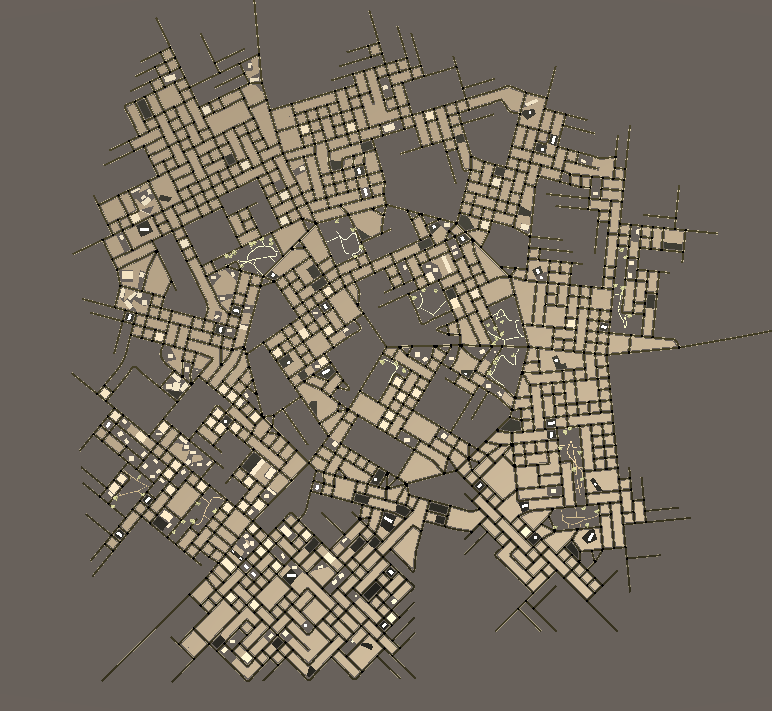
\includegraphics[width=\textwidth]{figure/discussion_city_layout_1}
  \end{subfigure}
  \quad
  \begin{subfigure}[b]{0.45\textwidth}
    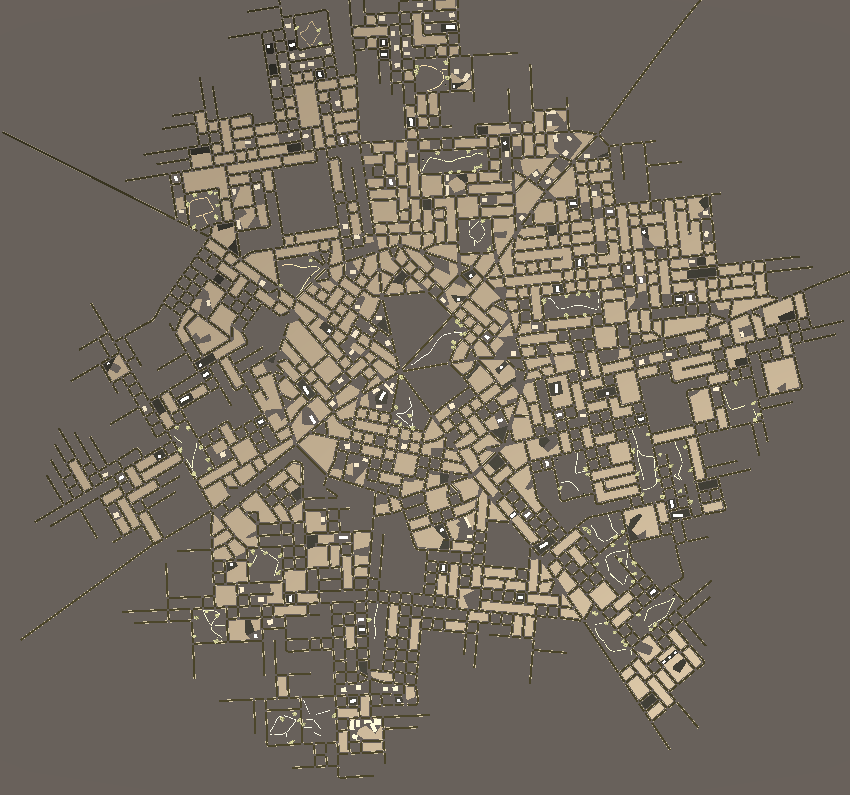
\includegraphics[width=\textwidth]{figure/discussion_city_layout_2}
  \end{subfigure}
  \caption{Two cities generated after consecutive runs under the same conditions highlighting the structural variety.}
  \label{fig:discussion_city_layout_variety}
\end{figure}

The variety in skyscrapers, buildings, and roads is limited though.
For example, roads always have the same appearance in terms of their cross-section and texture.
Buildings have some variety, but not close to those of reality.
Fortunately, the generation of buildings is versatile enough for more variety to be easily added.

% To what degree do the generated cities resemble real-world cities?
\textbf{Q4}:
When discussing the real-world resemblance of the generated cities mainly two things were considered.
These include the structural layout of the cities and whether the generated cities are believable in a real-world setting. 

The project group considers the structural layout of the Manhattan- and Paris-style cities to resemble their real-world counterparts to an acceptable degree.
This structural resemblance is demonstrated in the Figures~\ref{fig:road_network_manhattan \ref{fig:road_network_paris}.

As previously mentioned the pathways between roads, parking lots, and parks are impractical for human traversal which does not typically occur in reality.
Arguably such conditions can occur due to human error during construction that unsuccessfully accounts for human needs and accessibility.
To our knowledge, however, no real-world city exists that does not account for human convenience to the same degree as CityCraft.
In this regard, the project group does not consider the cities generated by CityCraft to be believable by real-world standards.

% How much control do the users have over the generation?
\textbf{Q5}:
The degree of control offered to the user is, with a few exceptions, at the level of supplying static settings to each sub-generator.
The exception to this is that the user can dynamically place individual cities and re-generate the content for each sub-generator.
This distinction highlights an important design choice of either creating a city editor with dynamic PCG, or a city generator capable of producing infinite worlds through static PCG.
CityCraft, tries to be both in the sense that each sub-generator is essentially stateless, but still imposes some user choices in the placement of cities for example.
Since the goal of CityCraft was to be a rough tool for generating cities that designers later could refine, the option for allowing the user to edit specific roads or alter the content of a selected block might not be deemed essential.
However, it would significantly improve designers' level of control.

% Are the cities suitable for use in digital media such as games and film?
\textbf{Q6}:
The cities generated by CityCraft are by no means mature enough for use in production quality digital media.
Some limiting factors include the texture quality and the odd gaps between roads and their surrounding buildings, parks and parking lots.
Although the generated cities might not be suitable as-is, CityCraft is still useful as a city prototyping tool as the cities can be generated in a short amount of time.
The cities could also be used as backdrops, as templates for further refinement, and of course research.

% Are users without technical expertise able to correctly use the application?
\textbf{Q7}:
When evaluating whether a user without any technical expertise would be able to correctly use the application, the project group concluded that such was the case.
This was concluded with the reasoning that all implementation details are irrelevant to the user.
Furthermore, the steps necessary to generate a city follow an easy step-by-step Wizard~\cite{yer_a_wizard} that is familiar to most users.
Admittedly, the application has not undergone any formal user testing to verify this.
One area of usability improvement would be to improve the design and pliancy of the user interface to provide better feedback.
For example, in the road generation step, the user might not notice that it is required to place a city marker to proceed.

% Are there any known crashes in the application or visual artifacts in the generated models?
\textbf{Q8}:
There is one significant bug and one crash known that might occur when using CityCraft.
% Placement of cities crash
The crash occurs under some unknown condition when placing city markers.
This rarely happens but is considered the most critical issue as it completely obstructs the user from using the application.
The bug is that the mesh generated for road intersections can sometimes become huge and cover a large part of the world.
The cause for this is known, however, due to the time limit has not been addressed properly.
In summary, the project group would consider CityCraft as stable given its development time.

\newpage